\section{Theorie}
\label{sec:Theorie}

Wird einem System, das aus Kondensator und Spule besteht, Energie zugeführt, so kann
diese Energie im System gespeichert werden, indem sie zwischen der Kapazität $C$
des Kondensators und der Induktivität $L$ der Spule hin und her schwingt. In der
Theorie kann dies verlustfrei geschehen, sodass sich eine ungedämpfte Schwingung
ergibt. In der Praxis ist dies allerdings nicht realisierbar, da jeder Leiter einen
Innenwiderstand besitzt und die Schwingung somit gedämpft wird. Zusätzlich kann auch
ein separater Widerstand $R$ in den Schwingkreis eingebaut werden. Mithilfe der Kirchhoff'schen
Regeln ergibt sich dann für diesen Schaltkreis \ref{fig:RLC}
\begin{equation}
  U_{\text{R}}(t)+U_{\text{C}}(t)+U_{\text{L}}(t)=0 \,.
\end{equation}

\begin{figure}
  \centering
  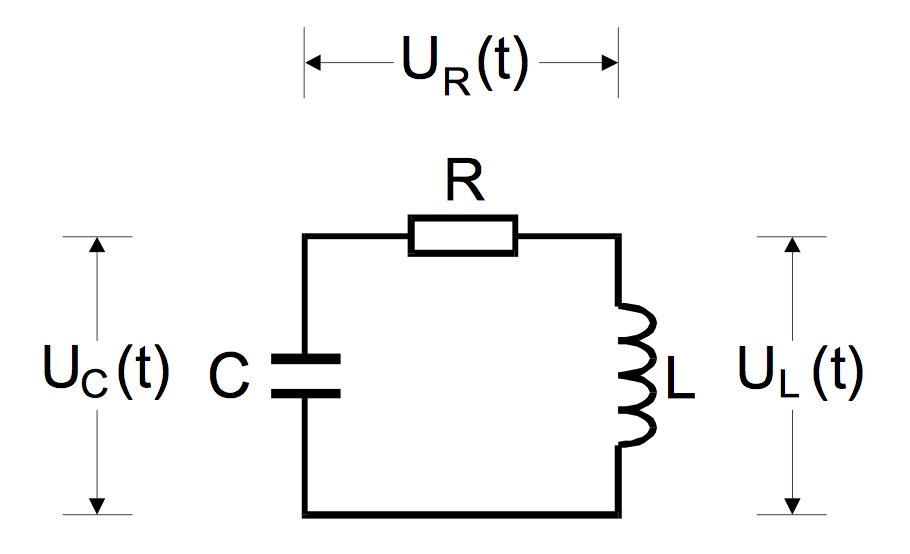
\includegraphics[width=300pt]{data/schwingkreis_theorie.png}
  \caption{Skizze eines RLC Kreises\cite{Versuchsanleitung1}}
  \label{fig:RLC}
\end{figure}

Werden nun die Beziehungen $U_{\text{R}}(t)=R \symbf{I}(t)$,
$U_{\text{C}}(t)=Q(t)/C$ und $U_{\text{L}}(t)=L (\symup{d} \symbf{I}/\symup{d}t)$
eingesetzt und wird nach der Zeit abgeleitet, so ergibt sich die Differentialgleichung
\begin{equation}
  \frac{\symup{d}^2\symbf{I}}{\symup{d}t}+\frac{R}{L}\frac{\symup{d}\symbf{I}}
  {\symup{d}t} + \frac{1}{LC}\symbf{I} = 0
\end{equation}
für gedämpfte Schwingungen. Zur Lösung kann der Ansatz
\begin{equation}
  \underline{\symbf{I}}(t)\footnote{Komplexe Zahlen werden im Folgenden mit einem
  Unterstrich markiert.}=\underline{U} \exp{i\underline{\omega}t}
\end{equation}
gewählt werden.
